\documentclass[letter,10pt]{article}
\usepackage[utf8]{inputenc}
\usepackage[spanish, activeacute]{babel}
\usepackage{geometry}
\geometry{verbose,tmargin=0cm,bmargin=2cm,lmargin=2cm,rmargin=2cm,headheight=0cm,headsep=1cm,footskip=1cm}
\usepackage{graphicx}


%%%%%%%%%%%%%%%%%%%%%%%%%%%%%% Textclass specific LaTeX commands.
\newcommand{\lyxaddress}[1]{
\par {\raggedright #1
\vspace{1.4em}
\noindent\par}
}

%%%%%%%%%%%%%%%%%%%%%%%%%%%%%% User specified LaTeX commands.
\date{}

\begin{document}

\title{Problema E - Escribiendo Mensajes}


\includegraphics[scale=0.6]{logo} \hspace*{9.00cm}

\includegraphics[scale=0.5]{dsc} 
\bigskip
\begin{center}
	\Large Problema E - Escribiendo Mensajes
\end{center}

\begin{flushright}
Límite de tiempo: 3 segundos
\par\end{flushright}
\bigskip

\section*{Problema}

El flojo fue víctima de un asalto, le robaron su celular y ahora tiene un viejo celular que tiene un teclado como el siguiente:

\begin{figure}[h!]
  \begin{center}
  	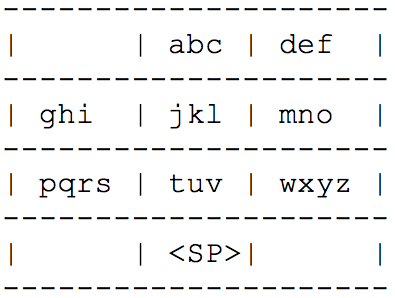
\includegraphics[scale=0.50]{mensaje}\caption{Teclado}
  \end{center} 
\end{figure}

Al flojo Mau no le gusta ese celular porque para escribir una letra tiene que presionar varias veces una misma tecla. Por ejemplo, para escribir la ``a'', él tiene que presionar la misma tecla una vez, pero para escribir la ``b'' tiene que presionar la misma tecla dos veces, y para la ``c'', tres veces. Para escribir un espacio, basta con presionar una vez la tecla $<$SP$>$.

El flojo Mau tiene que mandar un mensaje de texto con su celular, pero como es muy flojo no quiere mandar el mensaje si debe presionar muchas teclas. Tu tarea es ayudar a contar el número de teclas que el flojo Mau debe presionar para poder escribir un mensaje.

\subsection*{Entrada}

Un entero $T$, el número de casos de prueba. Las siguiente $T$ líneas contienen sólo espacios y caracteres en minúscula.

\subsection*{Salida}

Para cada caso de prueba debes imprimir una línea especificando el número del caso seguido del número de teclas que el flojo Mau debe presionar para escribir el mensaje de ese caso.

$$$$
$$$$
$$$$
$$$$
$$$$

\subsection*{Entrada ejemplo}
\noindent \texttt{2}~\\
\texttt{el flojo mau es muy flojo}~\\
\texttt{come frutas y verduras}~\\
\noindent 

\subsection*{Salida Ejemplo}

\noindent \texttt{Case \#1: 52}~\\
\texttt{Case \#2: 48}~\\

\noindent \rule[0.5ex]{1\columnwidth}{1pt}


\lyxaddress{UVA Online Judge}
\end{document}
